\begin{figure}[!htb]
  \centering
  \begin{subfigure}[b]{0.42\textwidth}
    \caption*{Squared Exponential Kernel}
  \end{subfigure}
  \begin{subfigure}[b]{0.42\textwidth}
    \caption*{Exponential Kernel}
  \end{subfigure}
  \hspace{0.05\textwidth}
  
  \begin{subfigure}[b]{0.14\textwidth}
    \caption*{$\rho = 0$}
  \end{subfigure}
  \begin{subfigure}[b]{0.14\textwidth}
    \caption*{$\rho = 0.5$}
  \end{subfigure}
  \begin{subfigure}[b]{0.14\textwidth}
    \caption*{$\rho = 1$}
  \end{subfigure}
  \begin{subfigure}[b]{0.14\textwidth}
    \caption*{$\rho = 0$}
  \end{subfigure}
  \begin{subfigure}[b]{0.14\textwidth}
    \caption*{$\rho = 0.5$}
  \end{subfigure}
  \begin{subfigure}[b]{0.14\textwidth}
    \caption*{$\rho = 1$}
  \end{subfigure}
  \hspace{0.05\textwidth}
  
  \begin{subfigure}[b]{0.14\textwidth}
    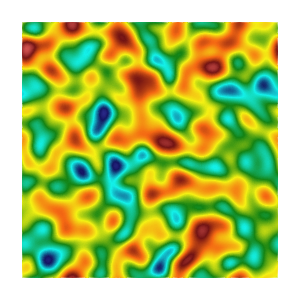
\includegraphics[width=\textwidth]{Chapter4/figures/2D/Gc_sqexp_cartesian_5_5_rho_1_sample_1.png}
    \caption{}
  \end{subfigure}
  \begin{subfigure}[b]{0.14\textwidth}
    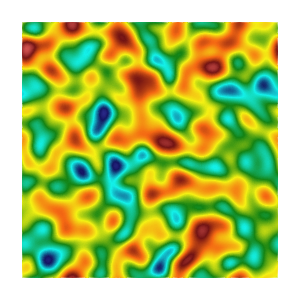
\includegraphics[width=\textwidth]{Chapter4/figures/2D/Gc_sqexp_cartesian_5_5_rho_1_sample_1.png}
    \caption{}
  \end{subfigure}
  \begin{subfigure}[b]{0.14\textwidth}
    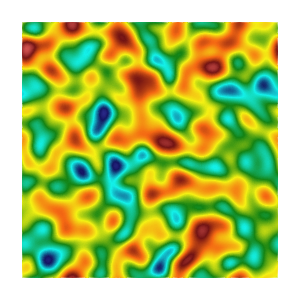
\includegraphics[width=\textwidth]{Chapter4/figures/2D/Gc_sqexp_cartesian_5_5_rho_1_sample_1.png}
    \caption{}
  \end{subfigure}
  \begin{subfigure}[b]{0.14\textwidth}
    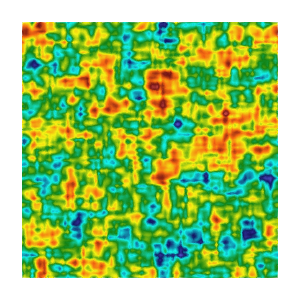
\includegraphics[width=\textwidth]{Chapter4/figures/2D/Gc_exp_cartesian_5_5_rho_1_sample_1.png}
    \caption{}
  \end{subfigure}
  \begin{subfigure}[b]{0.14\textwidth}
    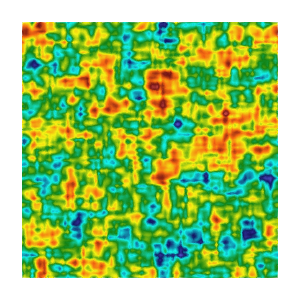
\includegraphics[width=\textwidth]{Chapter4/figures/2D/Gc_exp_cartesian_5_5_rho_1_sample_1.png}
    \caption{}
  \end{subfigure}
  \begin{subfigure}[b]{0.14\textwidth}
    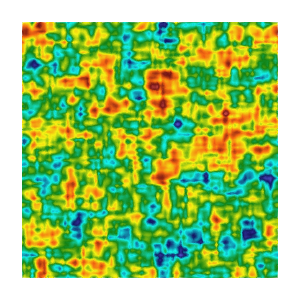
\includegraphics[width=\textwidth]{Chapter4/figures/2D/Gc_exp_cartesian_5_5_rho_1_sample_1.png}
    \caption{}
  \end{subfigure}
  \begin{subfigure}[b]{0.05\textwidth}
    \caption*{$\Gc^*$}
    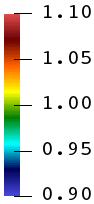
\includegraphics[width=\textwidth]{Chapter4/figures/rainbow_vertical.png}
    \vspace{0.05in}
  \end{subfigure}
  
  \begin{subfigure}[b]{0.14\textwidth}
    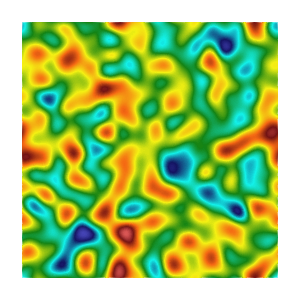
\includegraphics[width=\textwidth]{Chapter4/figures/2D/psic_sqexp_cartesian_5_5_rho_0_sample_1.png}
    \caption{}
  \end{subfigure}
  \begin{subfigure}[b]{0.14\textwidth}
    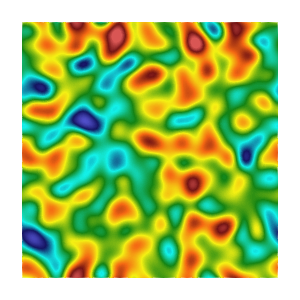
\includegraphics[width=\textwidth]{Chapter4/figures/2D/psic_sqexp_cartesian_5_5_rho_0_5_sample_1.png}
    \caption{}
  \end{subfigure}
  \begin{subfigure}[b]{0.14\textwidth}
    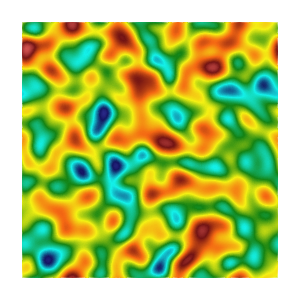
\includegraphics[width=\textwidth]{Chapter4/figures/2D/psic_sqexp_cartesian_5_5_rho_1_sample_1.png}
    \caption{}
  \end{subfigure}
  \begin{subfigure}[b]{0.14\textwidth}
    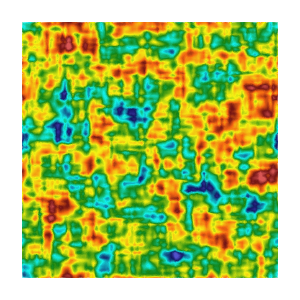
\includegraphics[width=\textwidth]{Chapter4/figures/2D/psic_exp_cartesian_5_5_rho_0_sample_1.png}
    \caption{}
  \end{subfigure}
  \begin{subfigure}[b]{0.14\textwidth}
    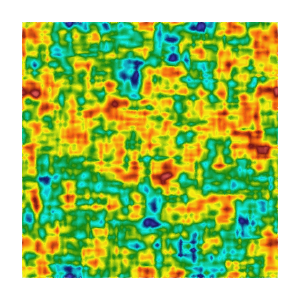
\includegraphics[width=\textwidth]{Chapter4/figures/2D/psic_exp_cartesian_5_5_rho_0_5_sample_1.png}
    \caption{}
  \end{subfigure}
  \begin{subfigure}[b]{0.14\textwidth}
    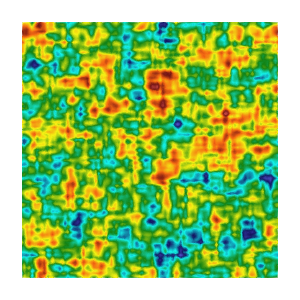
\includegraphics[width=\textwidth]{Chapter4/figures/2D/psic_exp_cartesian_5_5_rho_1_sample_1.png}
    \caption{}
  \end{subfigure}
  \begin{subfigure}[b]{0.05\textwidth}
    \caption*{$\psi_c^*$}
    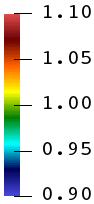
\includegraphics[width=\textwidth]{Chapter4/figures/rainbow_vertical.png}
    \vspace{0.05in}
  \end{subfigure}
  \caption[Point-wise correlated material properties with different covariance functions.]{ Point-wise correlated material properties: (a-f) normalized fracture toughness $\Gc^*$ and (g-l) normalized critical fracture energy $\psi_c^*$ with (left) PSE covariance function (right) PE covariance function }
  \label{fig: Chapter4/2D/compare_correlation}
\end{figure}
